\section{Extensions}
\label{section:extensions}

\subsection{Solver-specific improvements}
The main principles that drive the algorithm work regardless of which solver is used. However, the implementation can be improved by using more specific features of the solver.

\subsubsection{Indicator constraints}
Big M method: functional, but solvers struggle with large value of M. Low value of M -> may cause wrong behavior. Especially obvious when near vertical line. \\
Can approximate near vertical line as vertical line, but other solution is integer constraint from cplex. serves same role as big M method, but can't fail, is clearer and provides more information to solver.

\subsubsection{Max time}
When the MILP problem is sufficiently difficult to solve, it may take a long time before the solver can find the optimal solution. To ensure an upper limit on computation time, CPLEX accepts a maximum solve time parameter. When the maximum time has expired, it will return the best solution found so far.\\
In the experiments, the maximum solve time was typically 120 seconds per segment. The goal is for every segment to be relatively easy to solve, so if no solution can be found in two minutes it counts as a failure.
\subsubsection{Max delta}
During testing it became clear that the solver often spends a relatively long time trying to improve trajectories which are already nearly optimal, or optimal but not yet proven to be optimal. CPLEX provides a maximum delta parameter. The delta is the difference between the best solution found so far and the upper bound for the optimal solution. If the delta is below this maximum delta, the solvers stop executing and returns the best result. When this value is small, this can reduce some of the execution time while barely changing the quality of the trajectory.

\subsection{Corner cutting}
\begin{figure}
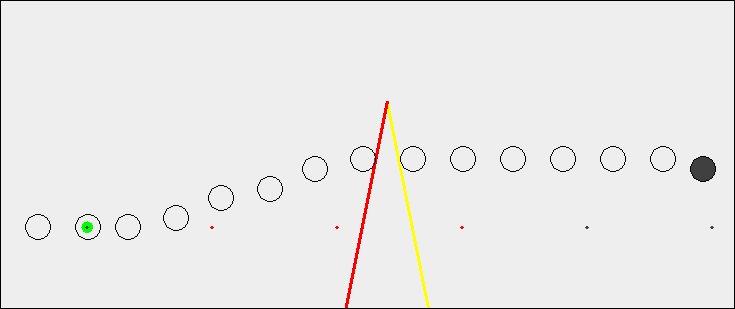
\includegraphics[width=\textwidth]{img/cornercut_bad}
\caption{An example of corner cutting}
\label{fig:cornercut-example}
\end{figure}
The MILP problem uses discrete time steps to model the changes in the UAV's state over time. An issue with this approach is that constraints are only enforced at those specific time steps. This allows the UAV to cut corners or even move through obstacles entirely if the vehicle is moving fast enough. Figure \ref{fig:cornercut-example} shows an example of this. Each time step on its own is a valid position, but a collision is ignored between the time steps.\\
As described in section (TODO: ADD REF), Equation \ref{eq:obs-repeat-1} and \ref{eq:obs-comb-repeat-1} prevent collisions with obstacle $o$ at time step $n$. Each edge of each obstacle has an associated $slack$ variable, which determines whether or not the UAV is on the safe side for that edge.
\begin{equation}
\label{eq:obs-repeat-1}
slack_{o,i,n} \Rightarrow \\
\begin{cases}
b_{o,i} \leq p_{n,y} - a_{o,i} p_{n,x} & dx_{o,i} < 0 \\
b_{o,i} \geq p_{n,y} - a_{o,i} p_{n,x} & dx_{o,i} > 0 \\
\end{cases}
\end{equation}
\begin{equation}
\label{eq:obs-comb-repeat-1}
\neg \mathlarger{\mathlarger{\bigwedge_{i}}} slack_{o,i,n} \quad 0 \leq n < N
\end{equation}
Richards and Turnbull\cite{Richards2015} proposed a method which prevents corner cutting. In their method, the UAV is consider on the safe side of an edge only if that is true for two consecutive time steps. They apply the same constraints again, but this time on the position of the UAV in the last time step:
\begin{equation}
\label{eq:corner-skip-fixed}
slack_{o,i,n} \Rightarrow \\
\begin{cases}
b_{o,i} \leq p_{n-1,y} - a_{o,i} p_{n-1,x} & dx_{o,i} < 0 \\
b_{o,i} \geq p_{n-1,y} - a_{o,i} p_{n-1,x} & dx_{o,i} > 0 \\
\end{cases}
\end{equation}
implemented simple version
TODO: implement more complex version
compare no vs simple vs complex


\subsection{Stability Improvements}

\subsubsection{Maximum goal velocity}
During segmentation

\subsubsection{GA start area}
not just path: stop point based on start state
stop point based on  maximum goal velocity and goal: ensures vehicle can stop in next segment

\subsubsection{Goal conditions}
larger epsilon on goal condition
prevent uav from finishing early -> use line

\subsection{Overlapping segment transitions}
overlap...

\subsection{Backtracking}
implement better!